\chapter[Validierung]{Validierung des multimodalen Modells}\label{cha:Evaluation}
Aus den gewonnen Interaktionszeiten der Studie modellierten wir ein multimodales Modell, mit deren Hilfe die Dauer multimodaler Interaktionen vorhergesagt werden kann.
Außerdem können verschiedene Kombinationen aus Modalitäten auf ihre Gesamtdauer verglichen werden. 

Im nächsten Schritt soll das erstellte multimodale Modell validiert werden. 
Dazu wollen wir in einer zweiten Studie die Gesamtdauer (Total Task Time) von multimodalen Interaktionen messen, um diese mit den Vorsagen des Modells vergleichen zu können. 

\section[Studienaufbau]{Studienaufbau}
Wir haben die Studie aufgeteilt in einen Übungsteil und in Anwendungsbeispiele, deren Gesamtdauer wir messen wollen. 
Der Übungsteil, enthält ausgewählte Anwendungsbeispiele aus Kombinationen von Modalitäten, die für den zweiten Teil benötigt werden. 
Mit diesen Übungen sollen sich die Probanden mit den Modalitäten vertraut machen. 
Im zweiten Teil sollen insgesamt fünf Anwendungsbeispiele getestet werden.
Für jedes Anwendungsbeispiel wurde eine Kombination von Modalitäten festgelegt. 

Für die Auswahl der fünf Anwendungsbeispiele haben wir die Kombination von Modalitäten explizit so gewählt, dass sie in ihrer Eignung besonders gut waren (siehe \fref{fig:Uebersicht_Eignung}) oder deren Kombination uns interessiert hat.
Die Texteingabe schnitt beispielsweise für die Sprachmodalität deutlich besser ab, als für die Touchmodalität, weshalb wir diese nur für Ersteres verwendeten.
Außerdem wollen wir auch Beispiele mit mehr als einem Modalitätswechsel testen. 

Das Modell wird nur stichprobenartig validiert, um die Studie in kürzerem Rahmen zu halten. 
Das heißt, dass in den Anwendungsbeispielen, die wir in der zweiten Studie testen werden, nicht alle modellierten Aktionen vorkommen. 

Die Studie zur Validierung unseres Modells fand unter gleichen Bedingungen statt; das heißt erneut bei BMW in Garching-Hochbrück am Parkring 19 in der Parkgarage im gleichen Studienfahrzeug (BMW 6er Gran Coupé). 
Das Auto wurde ans Stromnetz angeschlossen, um das Surface zu laden und eine dauerhafte Stromversorgung für Licht sowie Sitzheizung zu ermöglichen.
Das Surface wurde erneut am Dashboard und der Leap Motion Controller zwischen Gangschaltung und Dashboard angebracht. Die Einstellungen, der Aufbau des Prototypen, sowie die Protokollierung wurde wie in der ersten Studie vorgenommen. 

Die Einverständniserklärung, sowie den demographischen Fragebogen verwendeten wir gleichermaßen wie in der ersten Studie. 

Um in dieser Studie zusätzlich die subjektive Beanspruchung der Interaktionen zu messen, wurde der NASA Task Load Index (kurz NASA TLX) nach jedem Anwendungsbeispiel abgefragt \ref{cha:Anhang}. 
Der NASA TLX bewertet die subjektive Beanspruchung und unterscheidet dabei sechs Kategorien (Geistige Anforderung, Körperliche Anforderung, Zeitliche Anforderung, Leistung, Anstrengung und Frustration), die bewertet werden. 
Nach den fünf Anwendungsbeispielen wurde der zweite Teil des NASA TLX abgefragt, bei dem alle sechs Beanspruchungsvarianten miteinander verglichen (siehe \fref{sec:NASA_TLX}). 
Die 15 Vergleiche wurden für jeden Probanden in unterschiedlicher Reihenfolge abgefragt, um mögliche Einflüsse zu vermeiden. 
Außerdem wurde am Ende der Studie der INTUI Fragebogen vom Probanten aufgefüllt, um die Usability des Prototypen einzuschätzen; sowie drei Fragen in einem weiteren Fragebogen siehe \ref{cha:Anhang}. 
  
In den folgenden Unterabschnitten werden die Übungsbeispiele und die Anwendungsbeispiele erläutert.

\subsection[Übungsbeispiele]{Übungsbeispiele der Validierungsstudie}
In der Evaluationsstudie übt der Porbant befor er mit den Anwendungsbeispielen für die Evaluation beginnt. 
Dafür verwenden wir die Variante des Prototypen aus der ersten Studie. 
Die Anwendungsbeispiele sind dort kürzer und die Probanten können sich so mit den Interaktionen vertraut machen.
Wir haben folgende Übungsvarianten der ersten Studie ausgewählt (siehe \fref{fig:UseCases}):
\begin{enumerate}
	\item Navigation (Modalität: Geste und Sprache)
	\item Lautstärke (Modalität: Geste und Touch)
	\item Lautstärke (Modalität: Sprache und Geste)
	\item Temperatur (Modalität: Sprache und Touch)
	\item Telefon (Modalität: Touch und Sprache)
	\item Telefon (Modalität: Geste und Touch)
\end{enumerate}
Mit diesen Übungsbeispielen wurde die Direktauswahl aus sichtbaren Elementen (DA) mit Geste, Sprache und Touch geübt. 
Die Listennavigation (L) mit Sprache und Touch. 
Die direkte Inkrementation (Inkr. (d)) des Sliders mit Touch und Geste und zuletzt die schrittweise Inkrementation (Inkr.(s)) der Temperatureinstellung mit Touch. 
Dies deckt alle Interaktionen ab, die wir evaluieren werden. 

\subsection[Anwendungsbeispiele]{Anwendungsbeispiele der Validierungsstudie}
Nach dem Übungsdurchgang werden fünf Anwendungsbeispiele getestet werden. 
Dafür haben wir den multimodalen Prototypen angepasst. 
Er wird mit den gleichen Arten von Interaktionen bedient. 
Im Folgenden beschreiben wir die Anwendungsbeispiele und berechnen die multimodalen Interaktionszeiten, die mit Hilfe unseres Modell bestimmt werden.
 
Im Anwendungsbeispiel "`Lüftung"' soll die Lüftung auf Stufe 3 gestellt werden (siehe \fref{fig:UseCasesEvalLuft}). 
Dafür muss zuerst die Lüftungskachel mit dem Sprachbefehl "`Lüftung"' selektiert werden. 
Anschließend wird auf dem nächsten Screen mit drei Swipe-Touchgesten die Lüftung von 0 auf 3 gestellt. 
Der Wert wird nach einer kurzen Pause von selbst eingeloggt.  
\begin{figure}[ht]
	\centering
		\includegraphics[width=1\textwidth]{img/UseCases_Eval_Luft.jpg}
	\caption[]{Anwendungsbeispiel "`Lüftung"' mit den Modalitäten Sprache und Touch}
	\label{fig:UseCasesEvalLuft}
\end{figure}
Die Vorhersage der Interaktionsdauer mit dem multimodalen Modell wird wie folgt berechnet:
\[
\textbf{Lüftung} = \text{DA}_\text{S} + R(DA) + V(\text{Inkr.} (s))_\text{T} + 3*\text{Inkr.} (s)_\text{T}  + W_\text{ST} + R(\text{Screen}) =
\]
\[
= 2,795\text{s} + 0,5\text{s} + 0,906\text{s} + 3*0,547\text{s} +  0,273\text{s} + 0,016\text{s} = 6,133\text{s}
\]

Das Anwendungsbeispiel "`Lautstärke"' kennen wir bereits aus der ersten Studie. 
Hierbei soll die Lautstärke mit den Modalitäten Sprache und Geste von 50\% auf 80\% erhöht werden (siehe \fref{fig:UseCasesEvalMedienS}). 
Zuerst wird mit den Sprachbefehlen "`Medien"' und "`Lautstärke"' zweimal die Aktion Direktauswahl aus sichtbaren Elementen ausgeführt. 
Anschließend wird mit der direkten Inkrementation die Lautstärke verstellt. 
\begin{figure}[ht]
	\centering
		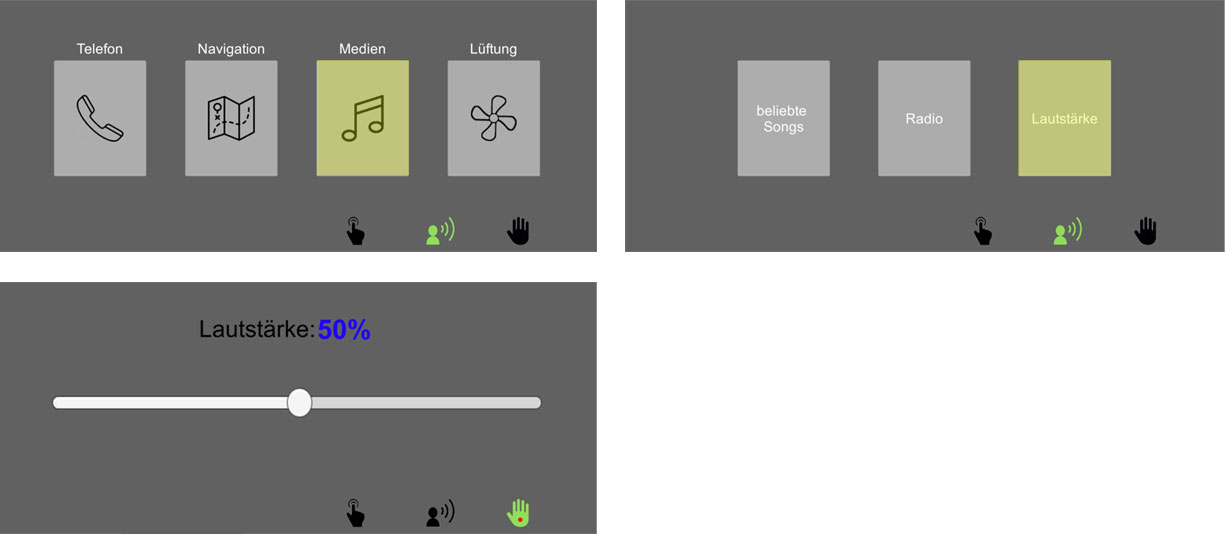
\includegraphics[width=1\textwidth]{img/UseCases_Eval_MedienS.jpg}
	\caption{Anwendungsbeispiel "`Lautstärke"' mit den Modalitäten Sprache und Touch}
	\label{fig:UseCasesEvalMedienS}
\end{figure}
Die Berechnung zur Vorhersage der Interaktionsdauer mit unserem Modell sieht wie folgt aus:
\[
\textbf{Lautstärke} = 2*(\text{DA}_\text{S} + R(DA)) + \text{Inkr.} (d)_\text{G} + W_\text{SG} + 3*R(\text{Screen}) =
\]
\[
= 2*( 2,795\text{s} + 0,5\text{s}) + 4,593\text{s} + 0,127\text{s} + 3*0,016\text{s} = 11,358 \text{s}
\]

Im Anwendungsbeispiel "`Medien"' soll zunächst per Geste die DA die Kachel "`Medien"' und "`beliebte Songs"' ausgewählt werden. 
Es erscheint eine Liste mit beliebten Songs. 
Mit dem Sprachbefehl "`Happy"' wird das Lied Happy abgespielt. 
Auf dem nächsten Screen, soll per Touch die Lautstärke geändert werden. 
Dafür wird der Lautstärke Button selektiert. 
Es erscheint ein Slider, der von 20\% auf 80\% ebenfalls per Touch geändert werden soll. 
Wird der Slider im Bereich zwischen 75\% und 85\% losgelassen erscheint ein Popup, dass noch per Touch bestätigt werden muss (siehe \fref{fig:UseCasesEvalMedien}).
\begin{figure}[ht]
	\centering
		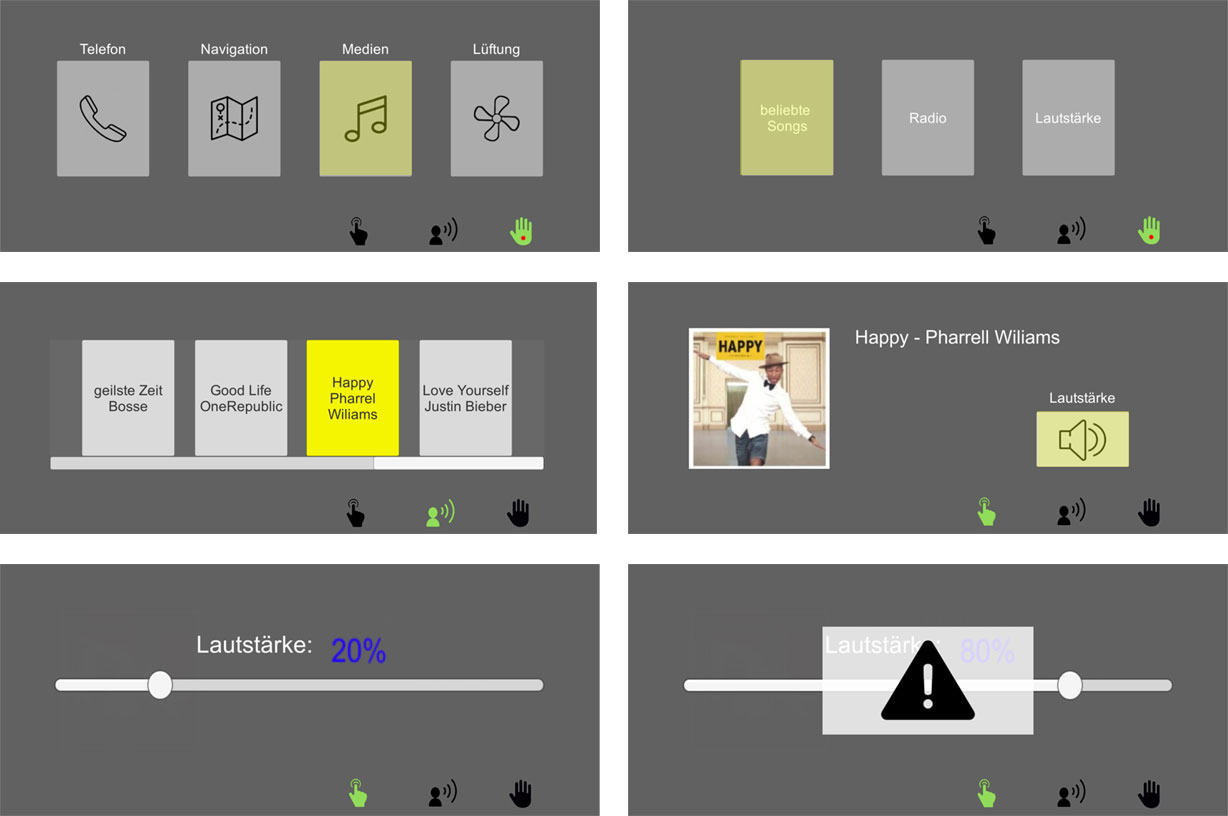
\includegraphics[width=1\textwidth]{img/UseCases_Eval_Medien.jpg}
	\caption{Anwendungsbeispiel "`Medien"' mit den Modalitäten Geste, Sprache und Touch}
	\label{fig:UseCasesEvalMedien}
\end{figure}
Die Vorhersage der Interaktionsdauer mit dem multimodalen Modell berechnet sich wie folgt:
\[
\textbf{Medien} = 2*(\text{DA}_\text{G}) + \text{Wort(m)}_\text{S} + W_\text{GS} + V(\text{1. Bu.})_T + \text{1-3 Bu.} + W_\text{ST} + 
\]
\[
 + Inkr.(d)_\text{T} + B_\text{T} + 6*R(\text{Screen}) =
\]
\[
= 2*( 2,436\text{s}) + 2,839\text{s} + 0,105\text{s} + 1,123\text{s} + 1,495\text{s} + 0,218\text{s} +
\]
\[
+2,795\text{s}+0,829\text{s} + 6*(0,016) = 15,014\text{s}
\]

Im Anwendungsbeispiel "`Navi POI"' wollen wir mit den Modalitäten Geste, Sprache und Touch den nächsten Coffeeshop finden. 
Dazu werden per Geste die Kacheln "`Navigation"' und "`Points of Interest"' ausgewählt. 
Anschließend erscheint ein Texteingabefeld zur Eingabe des POI. 
Mit dem Sprachbefehl "`Fastfood"' wird Fastfood in das Eingabefeld eingetragen. 
Erneut mittels Spracheingabe wird die Eingabe mit "`OK"' bestätigt. 
Jetzt wechselt der Screen zu einer Liste von Fastfood Geschäften. 
Es muss zur Kachel "`Starbucks"' auf der zweiten Seite mit der Touch-Eingabe geswiped werden. 
Auf der dritten Seite angekommen, muss noch die Kachel ausgewählt werden, siehe \fref{fig:UseCasesEvalNaviPOI}.  
\begin{figure}[ht]
	\centering
		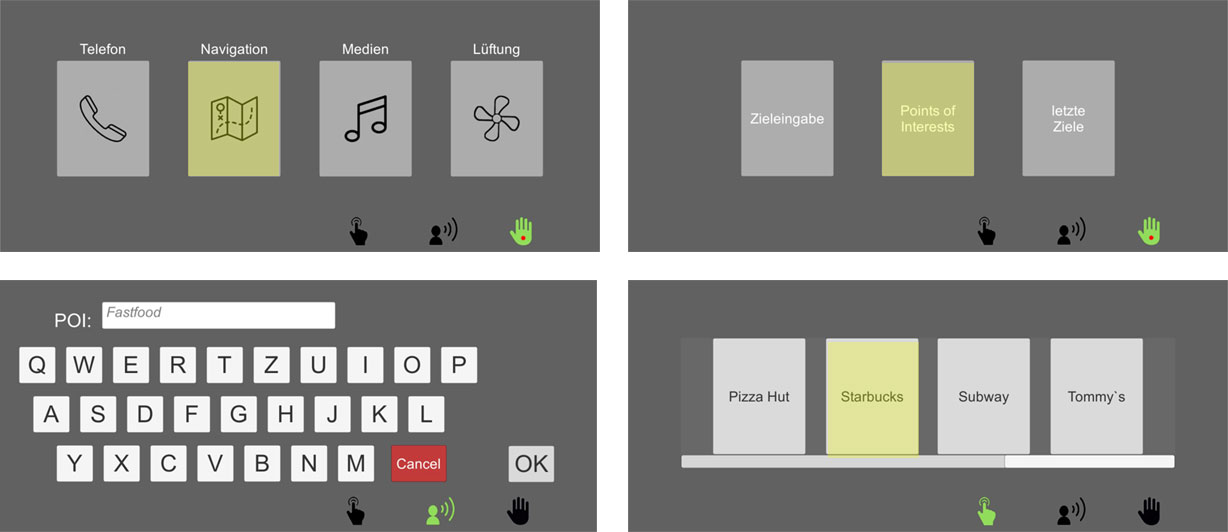
\includegraphics[width=1\textwidth]{img/UseCases_Eval_Navi_POI.jpg}
	\caption{Anwendungsbeispiel Navigation POI mit den Modalitäten Geste, Sprache und Touch}
	\label{fig:UseCasesEvalNaviPOI}
\end{figure}

In der ersten Studie haben wir festgestellt, dass die Positionierung des Eingabefeldes über der Tastatur besser geeignet ist, da somit die Hand nicht die Eingabe verdeckt.
Obwohl in unserer Kombination keine Touch-Eingabe verwendet wird, haben wir diese Anpassung bei den Screens mit Texteingabe vorgenommen.

Die Aktionsdauer dieses Anwendungsbeispiels wird folgendermaßen zusammengesetzt und berechnet:
\[	
\textbf{Navi POI} = 2*(\text{DA}_\text{G}) + \text{Wort(m)}_\text{S} + W_\text{GS} + B_\text{S} + 
\]
\[	
+ V(\text{L})_T + 2*(L)_T + W_\text{ST}(L_T) + DA(L)_T + 4*R(\text{Screen}) =
\]
\[
= 2*( 2,436\text{s}) + 2,839\text{s} + 0,105\text{s} + 1,972\text{s} + 
\]
\[
= + 0,705\text{s} + 2*0,813\text{s} + 1,495\text{s} + 0,375\text{s} + 1,047\text{s} + 4*0,016= 13,605\text{s}
\]

Im Anwendungsbeispiel "`Navigation Nummer"' soll zum Parkring 19 navigiert werden. 
Hier werden zwei Modalitäten (Touch und Sprache) mit insgesamt vier Moduswechseln verwendet. 
Per Touch werden die Kacheln Navigation und Zieleingabe gedrückt. 
Es wird das Texteingabefeld mit zwei Eingabefeldern (Straße und Hausnummer) geladen. 
Um das Eingabefeld "`Straße"' zu aktivieren, muss auf das entsprechende Eingabefeld getapt werden. 
Mit dem Sprachbefehl "`Parkring"' wird die Straße in das Eingabefeld eingetragen. 
Anschließend wird erneut mit einem Tap auf das Eingabefeld für die Hausnummer, dieses aktiviert. 
Mit dem Sprachebefehl "`19"' wird die 19 in das Eingabefeld eingetragen. 
Als letztes wird mit der Touch-Eingabe das Ziel mit dem "`OK"'-Button bestätigt (siehe (\ref{fig:UseCasesEvalNaviNummer}).
\begin{figure}[ht]
	\centering
		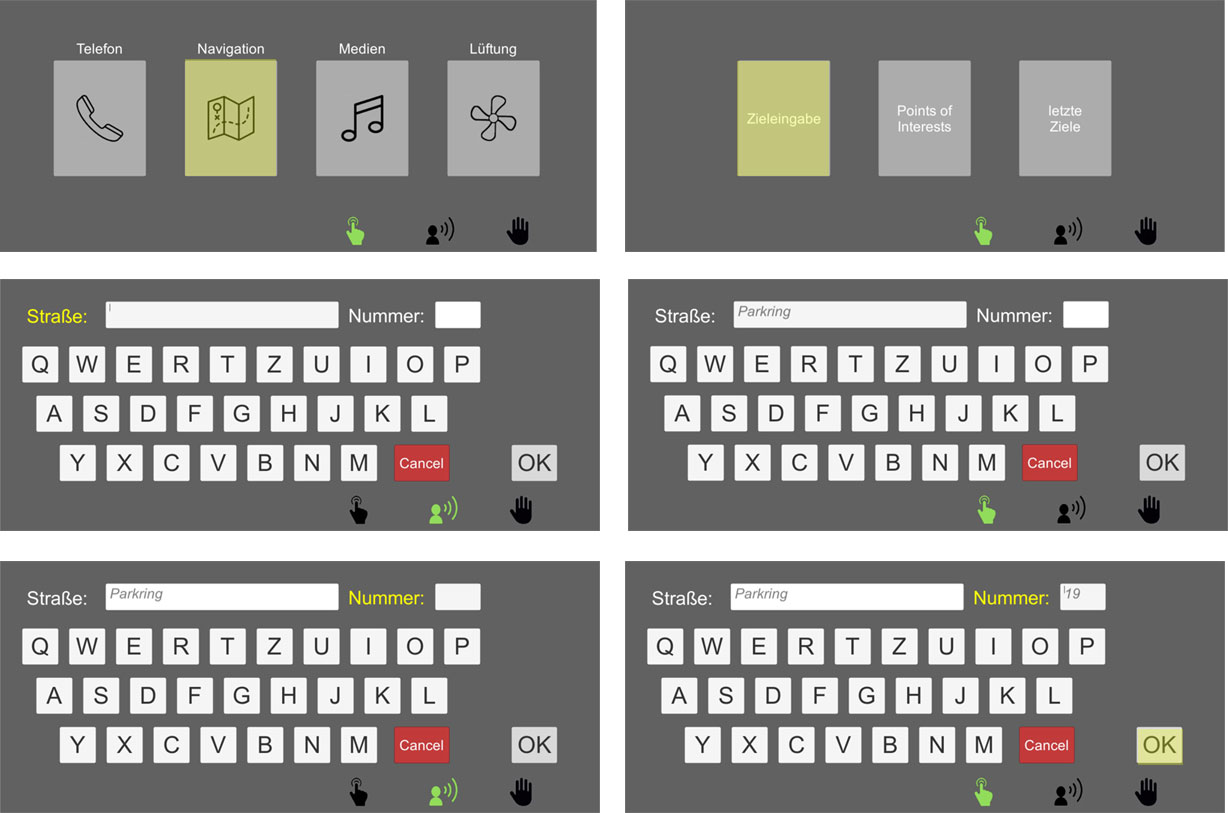
\includegraphics[width=1\textwidth]{img/UseCases_Eval_Navi_Nummer.jpg}
	\caption{Anwendungsbeispiel Navigation Nummer mit den Modalitäten Touch, Sprache, Touch, Sprache, Touch}
	\label{fig:UseCasesEvalNaviNummer}
\end{figure}	
Auch hier berechnen wir mit dem erstellten Modell die Interaktionsdauer:
\[
\textbf{Navi Nummer} = 2*(\text{DA}_\text{T}) + V(\text{1. Bu.})_T + \text{1-3 Bu.}_T + \text{Wort(m)}_S + W_\text{TS}(Wort(m)) +
\]
\[
+ V(\text{1. Bu.})_T + \text{1-3 Bu.}_T + W_\text{ST}(1. Bu.) + \text{Wort(m)}_\text{S} + W_\text{TS} + B_\text{T} + W_\text{ST} + 4*R(\text{Screen}) =
\]
\[
= 2*( 1,710\text{s}) +  1,123\text{s} + 0,642\text{s} + 2,839\text{s} + 0,079\text{s} + 1,123\text{s} + 
\]
\[
+ 0,642\text{s} + 0,218\text{s} + 2,839\text{s} + 0,079\text{s} + 0,642\text{s} + 1,123\text{s} + 0,218\text{s} + 3*0,016 = 15,035\text{s}
\]

\section[Studiendesign]{Studiendesign}
Auch in dieser Studie verwenden wir ein within-subject Design, in dem jeder Proband alle fünf Anwendungsbeispiele durchführen wird.
Unsere unabhängigen Variablen sind die fünf verschiedenen Anwendungsbeispiele, die unterschiedliche Aktionen in unterschiedlichen Modalitäten enthalten. 
Die abhängige Variable, die wir messen ist die Gesamtdauer in Sekunden, die ein Proband für jedes Anwendungsbeispiel benötigt. 

Die fünf Anwendungsbeispiele wurden mit dem Latin Square permutiert, um auch in dieser Studie mögliche Lerneffekte zu eliminieren.
Die Übungsbeispiele zu Beginn eines Studiendurchlaufs wurden jedoch in gleicher Reihenfolge durchlaufen. 

Die Vorhersage der Interaktionsdauer für unsere fünf Anwendungsbeispiele wird die Grundlage unserer Validierung sein. 
Wir werden die Zeiten der Anwendungsbeispiele messen, um diese mit unseren Vorhersagen vergleichen zu können. 

\section[Studienteilnehmer]{Studienteilnehmer}
Die Studiendauer eines Durchgangs betrug ca. 45 Minuten. In einem Zeitraum von zwei Tagen nahmen an der Evaluationsstudie insgesamt zehn Teilnehmer (acht männlich und zwei weiblich) teil. Das Alter erstreckte sich von 19-33 Jahren und betrug im Durchschnitt 23,8 mit einen Median von 22 Jahren, also etwas jünger als in unserer ersten Studie (Durchschnitt: 30,55 und Median: 25 Jahre). Alle zehn Teilnehmer sind Rechtshänder und sprechen deutsch als Muttersprache. 

Auch in der Evaluation wurde die Vorerfahrungen mit der Bedienung von Touch, Gesten und Sprache der Teilnehmer abgefragt und von den Probanden eingeschätzt.
Auf die Frage, ob sie Erfahrung mit der Bedienung von Sprache, Touch und Geste haben, konnte der Probant aus vier Optionen auswählen (1: nein, 2: ja, aber nur sehr wenig, 3: ja, benutze ich gelegentlich und 4: ja, benutze ich regelmäßig).
Die Vorerfahrung der Bedienung von Sprache ergab im Durchschnitt 3,1, bei Touch 4 und bei Geste 2,2.
Die Werte sind etwas höher als in unserer ersten Studie (Sprache: 2,32,  Touch: 3,95 und Geste: 1,86), was unter anderem daran liegen könnte, dass die Teilnehmer etwas jünger waren.

\section[Durchführung der Studie]{Durchführung der Studie}
Auch in dieser Studie wurde jeder Proband am Empfang am Parkrings 19 abgeholt und begrüßt.
Anschließend begaben wir uns in die Parkgarage zum Testfahrzeug, indem der Proband auf dem Fahrersitz platz nehmen sollte.
Er wurde darauf hingewiesen das Smartphone lautlos zu stellen und den Fahrersitz einzustellen.

Das Thema der Studie wurde kurz erläutert und darauf aufmerksam gemacht, dass zur Erhebung der Interaktionszeiten verschiedene Daten protokolliert werden und zusätzlich die Studie mit einer GoPro-Kamera aufgezeichnet wird.
Darüber aufgeklärt musste jeder Proband eine Einverständniserklärung unterschreiben (siehe Kapitel \ref{cha:Anhang}).
Zusätzlich sollte ein kurzer Fragebogen zu demografischen Daten und den Vorerfahrungen im Umgang mit den Interaktionen Touch, Geste und Sprache ausgefüllt werden.
In der Zwischenzeit startete der Studienleiter das Programm, stellte die richtige ID ein und überprüfte die neu geladene Permutation.

Die Vorgehensweise wurde Schritt für Schritt anhand der sechs Übungsbeispiele erklärt.
Die Probanten konnten sich somit mit den Interaktionen vertraut machen. 
Anschließend wurde die GoPro-Kamera gestartet, um die kommenden Anwendungsbeispiele für die Messung aufzunehmen.
Jedes Anwendungsbeispiel wurde zusätzlich in einem Probedurchlauf mindestens einmal geübt. 

Anschließend konnte mit dem ersten Messdurchgang begonnen werden. 
Nach jedem Messdurchgang wurde auch in dieser Studie auf einer 5-stufigen Likert-Skala abgefragt, wie geeignet die Probanden die Interaktion empfanden und wie sehr sie ihnen gefallen hat.
Traten während eines Messdurchgangs Fehler auf, wurde dies vom Versuchsleiter notiert, um den Protokolleintrag im Nachhinein als fehlgeschlagen markieren zu können. 
Fehlgeschlagene Messdurchgänge wurden wiederholt. 
Als fehlerhaft wurde ein Messdurchgang gewertet wenn zum Beispiel die Touch-, Gesten- oder Spracherkennung nicht richtig funktionierte oder wenn der Proband vergaß was er tun muss. 
\clearpage

\section[Auswertung der Studienergebnissen]{Auswertung der Studienergebnissen}
Im Folgenden werden nun die Ergebnisse der Evaluationsstudie präsentiert und diskutiert. 

\subsection[User Experience]{User Experience}
Im Vergleich zu Touch und Sprache war für die Teilnehmer die Gestensteuerung am ungewohntesten. 
Die Einschätzung der Eignung der Anwendungsbeispiele mit Geste schnitt nicht so gut ab wie die Anwendungsbeispiele ohne Geste.
Allerdings bekam das Anwendungsbeispiel "`Lautstärke"', indem der Lautstärkeslider mit einer Geste verstellt werden sollte, sehr positives Feedback (siehe \ref{fig:Smiley_Eignung_Gefallen}).
Hier wurde auf die Frage, ob ihnen die Interaktion gefallen würde nur eine negative Antwort gegeben.
Nach jedem Messdurchgang (also zwei pro Anwendungsbeispiel) sollten die Probanden auf einer Likertskala mit fünf Unterscheidungen angeben wie geeignet sie die Anwendung fanden und ob es ihnen gefallen hat.
\begin{figure}[ht]
	\centering
		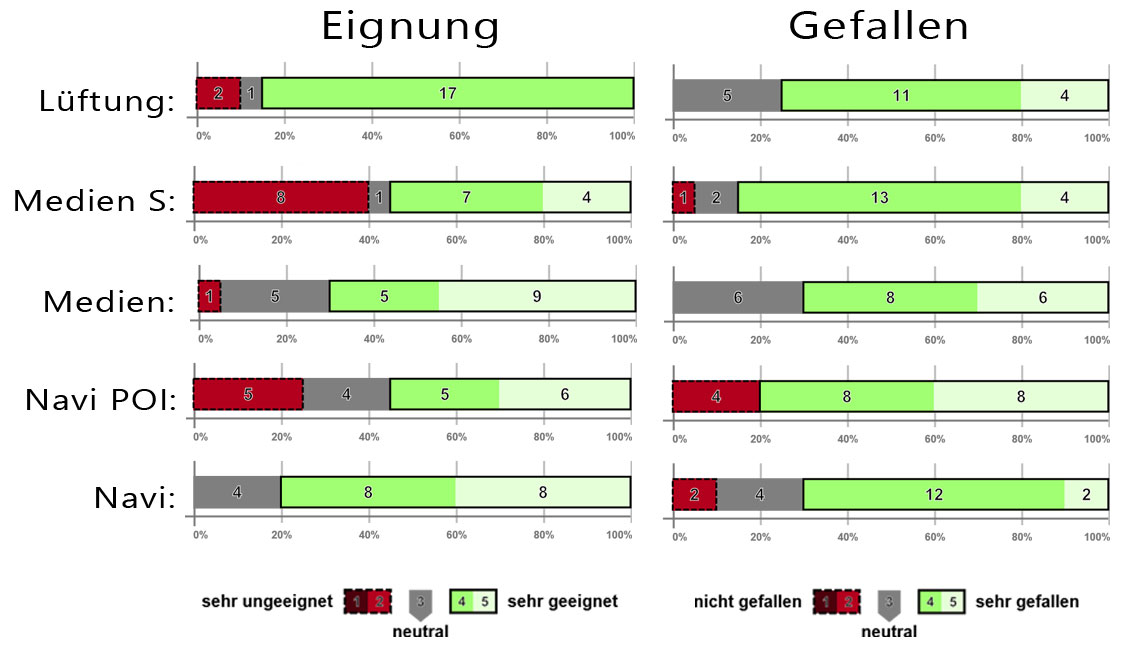
\includegraphics[width=1\textwidth]{img/Smiley_Eignung_Gefallen.jpg}
	\caption[Eignung und Gefallen der 5 Aufgaben]{Eignung und Gefallen der 20 Messdurchgänge der 5 Aufgaben. Die Balkendiagramme zur Darstellung von Likert-Skalen wurde mit http://likertplot.com/ generiert.}
	\label{fig:Smiley_Eignung_Gefallen}
\end{figure}
 
Neun von zehn Teilnehmern können sich eine multimodale Interaktion während dem Fahren vorstellen.
Begründet wurde dies mit der intuitive Bedienung, sowie vor allem dem Vorteil je nach Situation die passende Modalität frei wählen zu können.

Im INTUI Fragebogen (siehe Anhang im Kapitel \ref{cha:Anhang}) wurden verschiedene Komponenten der intuitiven Nutzung auf einer Skala von 1-7 abgefragt \citep{diefenbach2010handbuch}, \citep{ullrich2010intui}.
Die Probanden wurden hierfür darauf hingewiesen, dass sie sich dafür unseren Prototypen fehlerfrei vorstellen sollten, da unsere Umsetzung des Prototypen natürlich kein vollständig ausgearbeitetes Produkt ist.  
Die 17 Fragen mit verschiedenen Gegenüberstellungen werden vier Hauptbereichen zugewiesen (siehe \citep[Seite 24]{diefenbach2010handbuch}):
\begin{itemize}
\item \textbf{Mühelosigkeit (M):} Je höher der Wert, um so müheloser wird die Interaktion erlebt und desto weniger Aufmerksamkeit wird erfordert. Diese Komponente kann am ehesten mit der klassischen Usability verglichen werden.
\item \textbf{Bauchgefühl (G):} Je höher der Wert, um so weniger wird die Interaktion vom Verstand, sondern vom Gefühl geleitet. Diese Komponente ist "`eines der wichtigsten Merkmale intuitiver Entscheidungen in der Entscheidungspsychologie sowie im alltäglichen Sprachgebrauch"' \citep[Seite 24]{diefenbach2010handbuch}.
\item \textbf{Magisches Erleben (X):} Je faszinierender und außergewöhnlicher die Interaktion empfunden wurde desto höher ist dieser Wert. 
\item \textbf{Verbalisierungsfähigkeit (V):} Je höher der Wert, desto besser kann die Interaktion beschrieben werden. 
\end{itemize}
Die Ergebnisse des INTUI Fragebogens können aus \fref{fig:INTUI} entnommen werden.
\begin{figure}[ht]
	\centering
		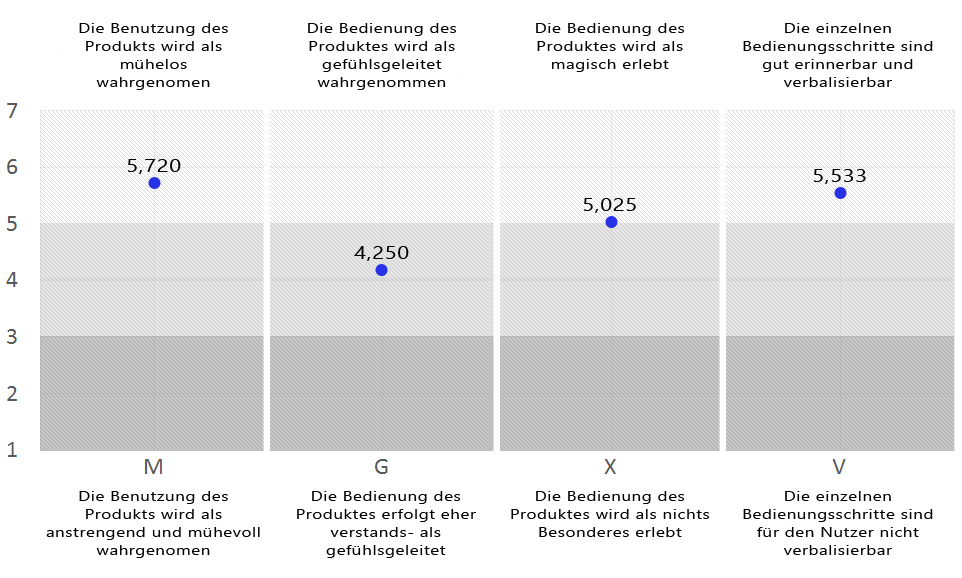
\includegraphics[width=1\textwidth]{img/INTUI_Grafik.jpg}
	\caption{Mittelwerte der vier Komponenten des INTUI Fragebogens}
	\label{fig:INTUI}
\end{figure}
Der extremste Wert ist mit 5,72 bei der Mühelosigkeit.
Das deutet auf eine gute Usability unseres Prototypen hin. TODO(aber sie sollten sich da produkt doch perfekt vorstellen, da kannst du jetzt nich credits fuer kassieren)
Beim Bauchgefühl zeigt der Wert eine minimale Tendenz zu einer gefühlsgeleitenden Interaktion hin. 
Der Wert des Magischen Erlebens mit 5,025 deutet auf eine außergewöhnliche Interaktion hin.
Die Abfolge unserer Bedienschritt schien unseren Probanden als einleuchtend, zumindest befindet sich der Wert der Verbalisierungsfähigkeit mit 5,533 im oberen Bereich.

\subsection{subjektive Belastung}
Beim NASA Task Load Index mussten sechs Beanspruchungskriterien auf einer Skala von 1-20 subjektiv von den Probanden bewertet werden.
Diese Werte werden alle mit 5 multipliziert, um eine Abstufung von 1-100 zu erhalten. 

Im zweiten Teil werden alle Kriterien miteinander verglichen und mit diesen 15 Vergleichen werden jetzt die Kriterien gewichtet.
Wurde die Frustration 4 mal vorgezogen erhält die Frustration eine Gewichtung (G) von 4.
Die Bewertung wird also mit 5 und dann mit deren Gewichtung multipliziert.
All diese Werte aufsummiert durch 15 geteilt ergeben den gesamten NASA TLX.
Diese Gewichtung führt dazu, dass für den Nutzer unwichtige Kriterien weniger bis gar nicht miteinbezogen werden und dafür wichtige um so mehr. 

Sei $B$ die Menge der Beanspruchungen, im Speziellen die Geistige Anforderung, Körperliche Anforderung, Zeitliche Anforderung, Leistung, Anstrengung und Frustration, dann sieht die Berechnung wie folgt aus:
\[
\textbf{NASA TLX} =\frac{1}{15}\sum_{i \in B}A_{i}G_{i}
\]
wobei $A_i$ der Wert der Beanspruchung ist und $G_i$ die Gewichtung.

Der durchschnittliche NASA TLX jedes Anwendungsbeispiels ist aus \fref{tab:PredictedVsObserved} zu entnehmen.
Das Anwendungsbeispiel "`Lüftung"' verursachte mit einem Wert von 25,6 die geringste Beanspruchung.
Am meisten beanspruchte das Anwendungsbeispiel "`Navigation Nummer"' mit den vier Moduswechseln und einem Wert von 37,533.
Wir stellen fest, dass mit Dauer der vorhergesagten Interaktionzeiten auch die durchschnittliche Beanspruchung zunimmt.

\subsection[Ergebnisse der Interaktionszeiten]{Interaktionszeiten im Vergleich zum multimodalen Modell}
Um unsere vorhergesagten Zeiten mit den beobachteten Zeiten vergleichen zu können berechnen wir den Root Mean Squared Error (RMSE). 
Der RMSE gibt uns an wie viele Sekunden die beobachteten Zeiten durchschnittlich von unserer Vorhersage abweichen.
Er wird wie folgt berechnet:
\[
RMSE = \sqrt{\frac{1}{n}\sum_{i=1}^{n}(r_i - p)^2}
\]
wobei $r_i$ unsere beobachteten Zeit von Proband $i$ (residuals) ist und $p$ die vorhergesagte Zeit.
Uns interessiert der prozentuale Fehler, also wird der RMSE noch durch unsere vorhergesagte Zeit geteilt.
Analog zu \citep{Card_1980} und \citep{schneegass_2009} verwenden wir eine logarithmische Skala um die vorhergesagten Zeiten unseres Modells mit den beobachteten Zeiten aus der Evaluation darzustellen. 

\fref{fig:predictedVsObserveredData} zeigt, dass sich unsere vorhergesagten Zeiten sehr gut mit den beobachteten Zeiten decken. 
\begin{figure}[ht]
	\centering
		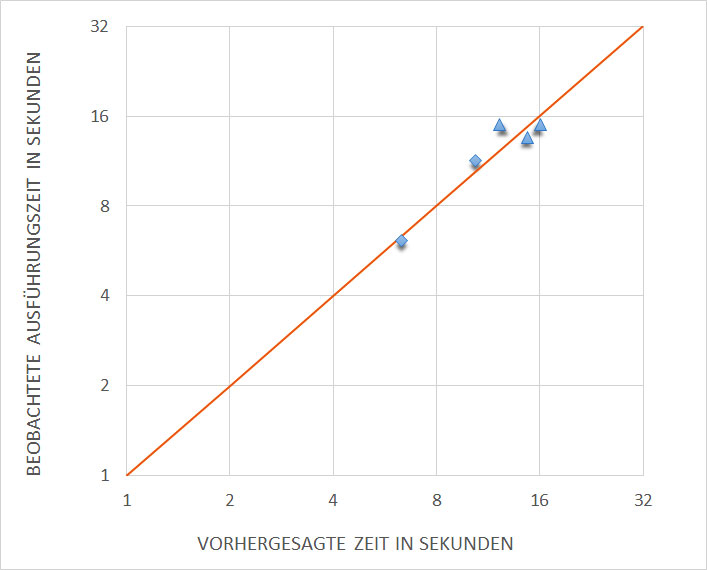
\includegraphics[width=1\textwidth]{img/predictedVsObserveredData.jpg}
	\caption[Übersicht der fünf Aufgaben im Vergleich zu den vorhergesagten und beobachteten Zeiten]{Übersicht der fünf Aufgaben im Vergleich zu den vorhergesagten und beobachteten Zeiten. Die Rauten sind Aufgaben mit nur einem Moduswechsel im Stil der ersten Studie. Die Dreiecke sind die Anwendungsbeispiele mit zwei und vier Moduswechseln.}
	\label{fig:predictedVsObserveredData}
\end{figure}

Der durchschnittliche prozentuale RMSE der fünf Anwendungsbeispiele beträgt 14,746\%, was deutlich geringer ist als die maximale Erwartung von 20-30\% \citep{Card_1980} und generell im guten Bereich von 5-20\% liegt \citep{Luo_2005}, \citep{Teo:2006}. 

\fref{tab:PredictedVsObserved} können die vorhergesagten Zeiten, die beobachteten Durchschnittszeiten, der RMSE in Sekunden und prozentual, sowie die durchschnittlichen Belastung des NASA TLX entnommen werden. 
\begin{table}[ht]
  \centering
		\begin{tabular}{|l|l|l|l|l|l|}
				\hline
				Aufgabe			& vorhergesagte 	& durchschnittliche 	& RMSE	& RMSE 		& Beanspruchung\\
				Modi (Wechsel)	& Zeit (s) 				& Zeit (s)						& (s)		& (\%) 		& NASA TLX 	 \\
				\hline
				Lüftung 			& 6,132						& 6,326 (+0,194)								& 0,864	&	14,098	&	25,600\\
				S,T (1)				&& 						&	&		&	\\
				\hline
				Lautstärke	& 11,36						&	10,413 (-0,947)							& 1,614 &	14,202	&	29,700\\
				S,G (1)				&& 						&	&		&	\\
				\hline
				Medien				& 15,014 					&	16,016 (+1,002)							& 1,860	&	12,389	&	33,100\\	
				G,S,T (2)			&& 						&	&		&	\\
				\hline
				Navi POI			& 13,605					& 14,682 (+1,077)							& 1,685	& 12,385	& 32,067\\
				G,S,T (2)			&& 						&	&		&	\\
				\hline
				Navi Nummer		& 15,035					& 12,215	(-2,82)						& 3,105 & 20,654	& 37,533\\		
				T,S (4)				&& 						&	&		&	\\
				\hline	
			\end{tabular}
	\caption[Vorhergesagte Werte im Vergleich zu beobachteten Werten]{Vorhergesagte Werte im Vergleich zu beobachteten Werten, deren RMSE in Sekunden und prozentual, sowie die durchschnittliche Beanspruchung des NASA TLX (Skala von 0-100).}
	\label{tab:PredictedVsObserved}
\end{table}

Unser Modell scheint auch für Interaktionen mit mehr als einem Moduswechsel anwendbar zu sein.
Gerade die Vorhersage der Anwendungsbeispiele "`Medien"' und "`Navigation POI"' mit je drei verschiedenen Modalitäten und somit zwei Modalitätswechsel ergeben die besten Ergebnisse mit einer Fehlerabweichung von nur 12,39\%. 

Die kompletten Ergebnisse aller zehn Probanden dieser beiden Anwendungsbeispiele sind in \fref{fig:Medien_Times} und \fref{fig:Navi_POI_Times} zu sehen. 

Für das Anwendungsbeispiel "`Medien"' liegen die Durchschnittszeit der Probanden über der vorhergesagten Zeit.
Ein Grund hierfür kann sein, dass für die Erhebung der Aktion Inkr. (d) eine Verschiebung von 50\% auf das Interval 75-85\% gemessen wurde.
In dem Evaluationsbeispiel sollte die Lautstärke von 20\% auf das Interval von 75-85\% gestellt werden.
Da hier die Spanne größer ist, könnte dieser Teil etwas länger gedauert haben. 

Auch beim Anwendungsbeispiel "`Navigation POI"' lag die vorhergesagte Zeit unter dem Durchschnitt. 
\begin{figure}[ht]
			\centering
			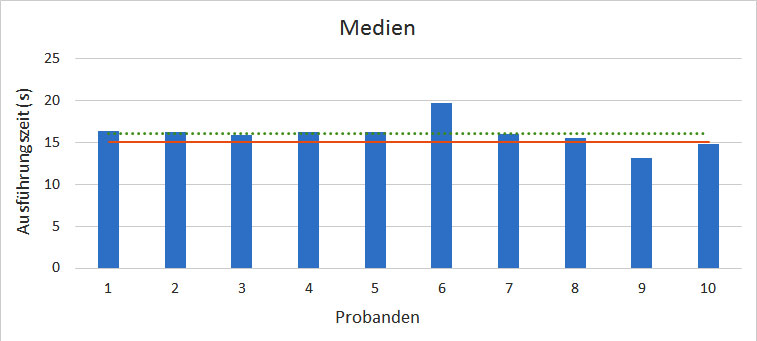
\includegraphics[width=1\textwidth]{img/Medien_Times.jpg}
			\caption[Zeiten der Probanden für das Anwendungsbeispiel "`Medien"'.]{Zeiten der Probanden für das Anwendungsbeispiel "`Medien"'. Enthält Modalitäten Geste, Sprache und Touch. Die rote durchgehende Linie stellt die vorhergesagte Zeit dar, die grüne gepunktete die Durchschnittszeit aller Probanden.}
			\label{fig:Medien_Times}
\end{figure}
\begin{figure}[ht]
			\centering
			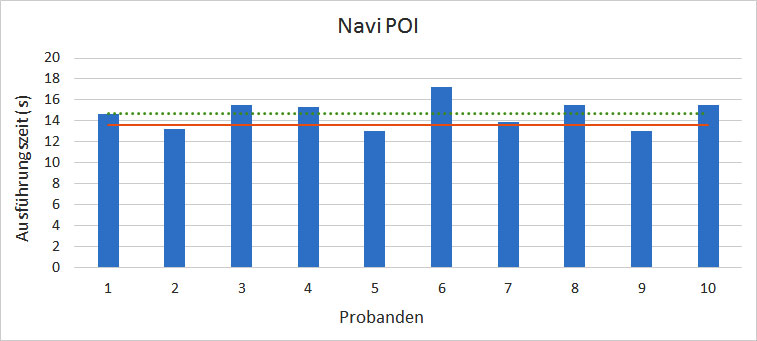
\includegraphics[width=1\textwidth]{img/Navi_POI_Times.jpg}
			\caption[Zeiten der Probanden für das Anwendungsbeispiel "`Navigation POI"'.]{Zeiten der Probanden für das Anwendungsbeispiel "`Navigation POI"'. Enthält Modalitäten Geste, Sprache und Touch. Die rote durchgehende Linie stellt die vorhergesagte Zeit dar, die grüne gepunktete die Durchschnittszeit aller Probanden.}
			\label{fig:Navi_POI_Times}		
\end{figure}

Die Anwendungsbeispiele "`Lüftung"' und "`Lautstärke"' waren fast identisch zu den Beispielen der ersten Studie.
Diese hatten beide nur einen Moduswechsel.
Beim Anwendungsbeispiel "`Lüftung"' liegt unsere Vorhersage unter dem Durchschnitt.
Das Anwedungsbeispiel "`Lautstärke"' liegt unsere Vorhersage allerdings über dem Durchschnitt. 
Das ist eventuell der Tatsache zu schulden, dass die Probanden der Evaluationsstudie insgesamt besser mit der Slidegeste für die Einstellung des Lautstärkesliders zurecht kamen. 
Die kompletten Ergebnisse aller zehn Probanden dieser beiden Anwendungsbeispiele sind in \ref{fig:Luft_Times} und \ref{fig:MedienS_Times} zu sehen. 
\begin{figure}[ht]
			\centering
			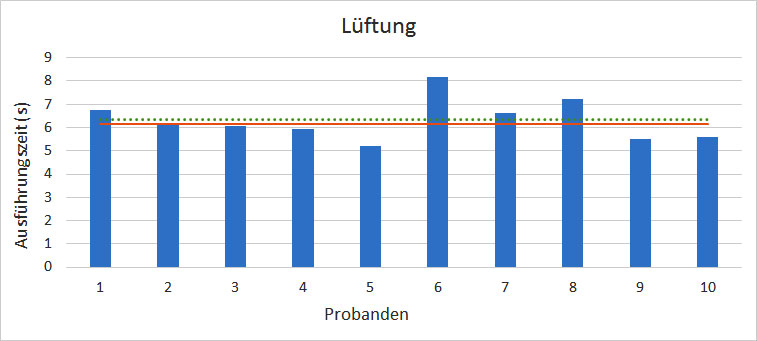
\includegraphics[width=1\textwidth]{img/Luft_Times.jpg}
			\caption[Zeiten der Probanden für das Anwendungsbeispiel "`Lüftung"'.]{Zeiten der Probanden für das Anwendungsbeispiel "`Lüftung"'. Enthält Modalitäten Sprache und Touch. Die rote durchgehende Linie stellt die vorhergesagte Zeit dar, die grüne gepunktete die Durchschnittszeit aller Probanden.}
			\label{fig:Luft_Times}
\end{figure}
\begin{figure}[ht]
			\centering
			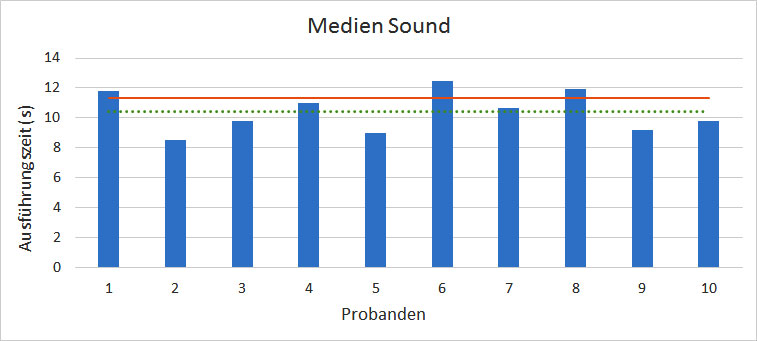
\includegraphics[width=1\textwidth]{img/Medien_S_Times.jpg}
			\caption[Zeiten der Probanden für das Anwendungsbeispiel "`Lautstärke"'.]{Zeiten der Probanden für das Anwendungsbeispiel "`Lautstärke"'. Enthält Modalitäten Sprache und Geste. Die rote durchgehende Linie stellt die vorhergesagte Zeit dar, die grüne gepunktete die Durchschnittszeit aller Probanden.}
			\label{fig:MedienS_Times}		
\end{figure}

Das Anwendungsbeispiel "`Navigation Nummer"' schnitt mit einem prozentualen RMSE von 20,654\% am schlechtesten ab.
Mit zwei verschiedenen Modalitäten und vier Modalitätswechseln ist dies das aufwändigste Beispiel.
Für die Aktivierung der Eingabefelder verwendeten wir in unserem Modell zur Vorhersage die Zeit die benötigt wird um den ersten Buchstaben zu drücken.
In jetzigen Beispiel ist die Touchfläche allerdings deutlich größer als die Touchfläche der Buchstaben aus der ersten Studie.
Nach Fitts` Law \citep{fitts1954information}, \citep{sasangohar2009evaluation} beeinflusst die Größe der Touchfläche $W$ die Interaktionszeit positiv.
Es erschien es uns besser die Interaktionszeit zu überschätzen, als zu unterschätzen.
Es lässt sich in diesem Beispiel gut erkennen, das unsere Vorhersage für alle Probanden zu groß waren (siehe \fref{fig:Navi_Times}).
\begin{figure}[ht]
	\centering
		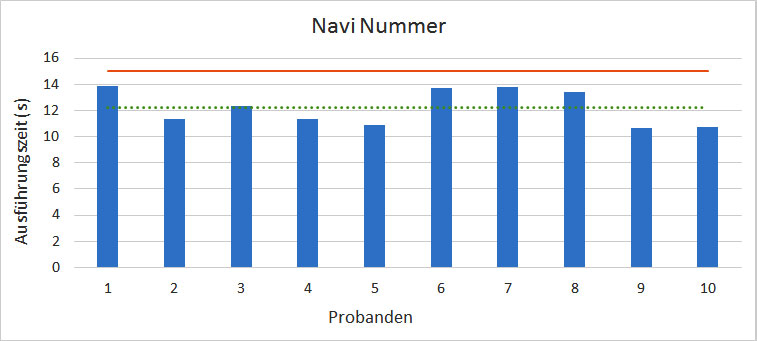
\includegraphics[width=1\textwidth]{img/Navi_Times.jpg}
	\caption[Zeiten der Probanden für das Anwendungsbeispiel "`Navigation TODO"'.]{Zeiten der Probanden für das Anwendungsbeispiel "`Navigation TODO"'. Enthält Modalitäten Touch, Sprache, Touch, Sprache und Touch. Die rote durchgehende Linie stellt die vorhergesagte Zeit dar, die grüne gepunktete die Durchschnittszeit aller Probanden.}
	\label{fig:Navi_Times}
\end{figure}

\subsection{Vergleich des Modells ohne Wechselkosten}
Im multimodalen Modell zur Vorhersage von Interaktionszeiten, sind die Wechselkosten zwischen zwei Modalitäten ein wichtiger Bestandteil. 
Uns interessiert, welchen Einfluss diese Wechselkosten für die Vorhersage von multimodalen Interaktionszeiten haben. 
Dafür vergleichen wir die Interaktionszeiten des erstellten multimodalen Modells mit den Interaktionszeiten, die ohne die Berücksichtigung von Wechselkosten entstehen.
Der durchschnittliche prozentualen RMSE für alle fünf Anwendungsbeispiele, ohne Berücksichtigung der Wechselkosten, liegt bei 15,561\%; der durchschnittliche prozentualen RMSE von dem multimodalen Modell mit Wechselkosten bei 14,746\%. 
\begin{figure}[ht]
	\centering
		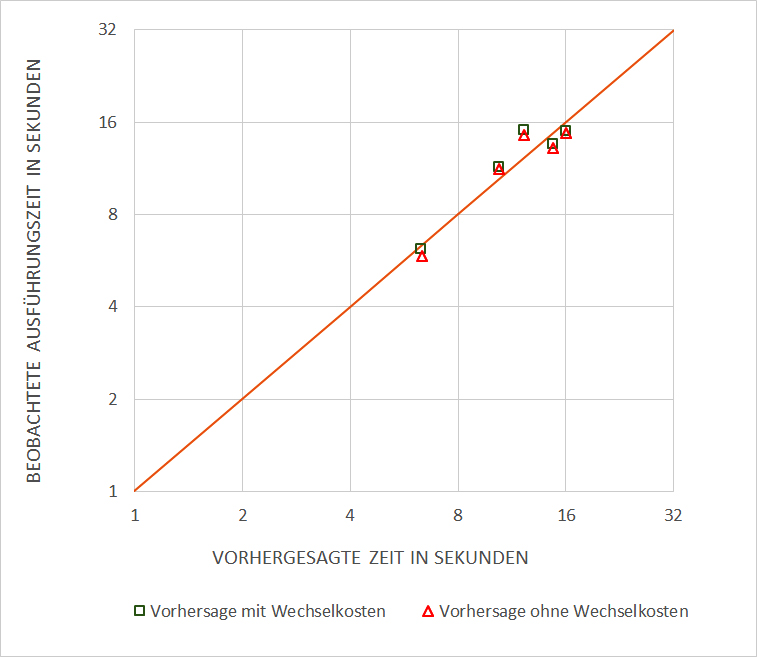
\includegraphics[width=1\textwidth]{img/Vorhersagezeit_ohne_Wechselkosten.jpg}
	\caption[Interaktionszeiten ohne Wechselkosten]{Vorhersage ohne Wechselkosten im Vergleich}
	\label{fig:Vorhersagezeit_ohne_Wechselkosten}
\end{figure}
\fref{fig:Vorhersagezeit_ohne_Wechselkosten} gibt die Unterschiede der beiden Modelle wieder. 
Die Anwendungsbeispiele, bei denen die tatsächliche Zeit über der Vorhersage lag, nähern sich jetzt näher an die Vorhersage an, da die Zeiten kürzer werden.
In den drei Anwendungsbeispielen, die unter der geschätzten Zeit lagen entfernen sich weiter. 
Obwohl sich der durchschnittliche prozentuale RMSE ohne Berücksichtigung der Wechselkosten auf 15,561\% verschlechtert hat, gibt es keine signifikanten Unterschiede.
 
\clearpage
\section[Diskussion]{Diskussion}
Die Evaluierung unseres multimodalen Modells soll nun mit Hinblick auf die Ergebnisse diskutiert und mit Ergebnissen aus anderen Arbeiten verglichen werden.
Des Weiteren gehen wir auf qualitative Erkenntnisse ein, die sich aus beiden Studien durch Kommentare und Beobachtungen ergeben haben.

\subsection[Modell]{Multimodales Modell}
Die fünf evaluierten Anwendungsbeispiele ließen sich mit unserem Modell mit einem durchschnittlichen prozentualem RMSE von 14,746\% vorhersagen.
Dieser durchschnittliche prozentuale RMSE befindet sich sowohl im Bereich von 20-30\% den \citet{Card_1980} als maximalen Fehler empfiehlt, als auch im Bereich von 5-20\% \citep{Luo_2005,Teo:2006}. 
In diesen Arbeiten werden die Interaktionszeiten allerdings auf der Grundlage eines Keystroke-Level-Modells oder deren Erweiterung auf Operatorebene berechnen. 
Davon ausgehend, dass unser Modell grobgranularer aufgebaut ist als das Keystroke-Level-Modell, stellt sich unser Modell zur Vorhersage von multimodalen Interaktionen als vielversprechend Methode heraus. 

Die subjektive Bewertung der Nutzer durch den NASA TLX ihrer Beanspruchung während der multimodalen Interaktion lag zwischen 25,6 und 37,533 auf einer Skala von 0-100. 
Den geringsten Beanspruchungswert von 25,6 hatte das Anwendungsbeispiel "`Lüftung"' mit den Modalitäten Sprache und Touch mit einem Modalitätswechsel. 
Es lässt sich erkennen, dass die Beanspruchung mit der vorhergesagten Interaktionsdauer zunahm.
Der höchste Wert von 37,533 wurde im Anwendungsbeispiel "`Navigation Numer"' erreicht. 
Dieses Anwendungsbeispiel hatte insgesamt 4 Modalitätswechsel zwischen Touch und Sprache.  

Die beliebtesten Kombinationen von Modalitäten der 22 Nutzer aus der ersten Studie waren die unimodale Variante mit Sprache. 
Am zweit beliebtesten war die Kombination von Touch und Sprache. 
Die dritt beliebteste Variante war die Kombination von Geste und Sprache. 
Das deutet darauf hin, dass multimodale Interaktionen von den Nutzern akzeptiert und sogar gern benutzt wird. # oder einfach nur dass sie Sprache moegen 
Aus dem Fragebogen der zweiten Studie kam heraus, dass neun von zehn Teilnehmern sich eine multimodale Interaktion, im Stile unserer Evaluationsstudie, während dem Fahren vorstellen könnten. 
Die intuitive Bedienung, sowie dem Vorteil sich je nach Situation die passende Modalität frei wählen zu können kommt bei den Nutzern gut an. 
Jedoch bleibt in diesem Feld der multimodalen Interaktion noch viel zu forschen und verbessern, bis die Erwartungen und Vorteile vollends ausgeschöpft werden können.

Das Design unseres Prototypen wurde Anhand der im Workshop (Connected Minds) gewonnenen Informationen über Interaktionen im Auto modelliert. 
Wir mussten uns auf bestimmte Gesten einigen, die uns am sinnvollsten für unsere Aktionen erschienen. 
Es gibt jedoch andere Varianten, die ebenfalls als Aktionen in Frage kommen. 
Zum Beispiel die kreisförmige Geste mit dem Zeigefinger nach links oder rechts, um die Lautstärke zu verringern oder zu erhöhen. 
Eine Geste dieser Art ist bereits im BMW 7 Series eingebaut.
Die Erkennung dieser Geste vom Leap Motion Controller ist noch nicht gut genug, weshalb wir uns dort eine andere Variante überlegten.

Ein weiterer Mangel unseres Modell sind die schon erwähnten, fehlenden haptischen Bedienelemente. 
Diese sind natürlich ein wichtiger Bestandteil und sollten als weitere Modalität in unser Modell miteinbezogen werden. 

Bei der Aktion Inkr. (d) wurde in der ersten Studie zur Erhebung der Interaktionszeiten lediglich der Slider von 50\% auf 75-85\% verstellt.
Für unsere grobe Betrachtung erschien uns diese Einstellung als ausreichend zur Bestimmung dieser Interaktionszeit. 
Da in dem Anwendungsbeispiel der Evaluation jedoch die Zeiten für eine Verstellung von 20 auf 75-85\% länger dauerte, sollte diese Aktion eventuell genauer untersucht werden. 

Die Ergebnisse des INTUI Fragebogens für die Mühelosigkeit, deuten auf eine gute Usability unseres Prototypen hin. 
Ein Grund dafür kann an dem vereinfachten und abstrakten Design liegen, das gewählt wurde um nicht unnötig abzulenken.
Der multimodale Prototyp wurde nur zur Erhebung der Interaktionszeiten entwickelt und bildetet kein komplettes Informationssystem im Fahrzeug ab. 
Deshalb konnte auf viel Informationsinhalt verzichtet werden, was den Prototypen übersichtlicher und leichter zu bedienen macht.
Auch der durchschnittliche Wert des Magischen Erlebens mit 5,025 von 7 deutet auf eine außergewöhnliche Interaktion hin. 
Dies liegt wahrscheinlich an der multimodalen Interaktion und vor allem an der Gesteninteraktion, die für viele neu war. 
Die Abfolge unserer Bedienschritt schien unseren Probanden als einleuchtend, zumindest befindet sich der Wert der Verbalisierungsfähigkeit mit 5,533 im oberen Bereich.

\subsection[Qualitative Erkenntnisse]{Qualitative Erkenntnisse}
Während beider Studien zur Bedienung eines multimodalen Interface im Auto ist aufgefallen, dass der Bereich von Gesteninteraktionen sehr individuell von der Sitzeinstellung und Armlänge abhängt.
Am ergonomisch geeignetsten hatten es die Nutzer, die ihren Arm an der Armlehne ablegen konnten und sich trotzdem mit der Hand im gewünschten Interaktionsbereich befanden. 
Für zukünftige Gestensteuerung im Auto sollte dies berücksichtigt werden, um verkrampfte und unnatürliche Bewegungen zu reduzieren.
Zum Beispiel könnte durch eine verstellbare Armlehne, sowie einen anpassbaren Interaktionsbereich zur Gestenerkennung die optimale Einstellung erreicht werden.
Dies ermöglicht nicht nur eine bequemere Gesteninteraktion, sondern reduziert auch mögliche Erkennungsfehler von Gesten, was wiederum zu einer besseren User Experience führt.

Der Touchbereich war ebenfalls für manche Nutzer nur gut zu Erreichen, indem sie sich etwas vor lehnten.
Sie  wurden angewiesen sich vor der Studie den Sitz so einzustellen als würden sie fahren, doch trotz diesen Vorkehrungen war der Touchdisplay nicht für alle optimal positioniert.
Auch in der Touchbedienung gibt es noch Potenzial zur Verbesserung.
Die Position des Touchbereichs sollte näher am Fahrer liegen, als bei Informationssystemen im Auto ohne Touchdisplays.
